\chapter{Konzeption des Systems}
\label{chap:konzeption}

\section{\"Uberblick}
Die Konzeption des Systems bildet das Fundament für die spätere Implementierung und vereint moderne Technologien, um eine leistungsfähige und benutzerfreundliche Mitarbeitergesprächssoftware zu entwickeln. Im Zentrum der Konzeption stehen drei essenzielle Bereiche: das Design, die technischen Komponenten und die Datenarchitektur.

Das System zielt darauf ab, durch die Kombination von Frontend-Technologien wie React und Vite mit einem effizienten Backend auf Basis von .NET Core eine skalierbare und zuverlässige Plattform zu schaffen \cite{kirk2016data, microsoftDotNet}. Ergänzt wird dies durch eine relationale Datenbankstruktur, die mit Azure SQL realisiert wird, um eine robuste und sichere Speicherung sowie Verarbeitung der Gesprächsdaten zu gewährleisten \cite{azureDocumentation}.

Ein besonderer Fokus liegt auf der Interoperabilität mit bestehenden HR-Infrastrukturen. Durch den Einsatz von Microsoft Azure-Diensten wie Active Directory und Microsoft Graph wird eine nahtlose Integration ermöglicht, die nicht nur die Benutzerfreundlichkeit steigert, sondern auch die Effizienz datenbasierter Entscheidungsprozesse fördert \cite{microsoftAzure}. Die Architektur ist darauf ausgelegt, Visualisierungstools wie Donut- und Radarcharts zu integrieren, die eine intuitive und präzise Darstellung komplexer Daten unterstützen \cite{evergreen2016effective}.

Diese Konzeption stellt sicher, dass die verschiedenen Komponenten des Systems harmonisch zusammenwirken, um den Anforderungen moderner Arbeitsumgebungen gerecht zu werden und gleichzeitig die Grundlage für eine zukunftssichere Weiterentwicklung zu schaffen.


\section{Systemarchitektur}
Die Systemarchitektur basiert auf einem klassischen Client-Server-Modell, das eine klare Trennung zwischen der Benutzeroberfläche und den serverseitigen Prozessen gewährleistet. Diese Architektur erlaubt eine modulare und skalierbare Entwicklung, die sowohl Benutzerfreundlichkeit als auch Systemeffizienz priorisiert.

Das Frontend wird mit React entwickelt, einer modernen JavaScript-Bibliothek, die durch ihre komponentenbasierte Struktur eine effiziente Erstellung und Wiederverwendbarkeit von Benutzeroberflächen ermöglicht \cite{stefanov2021react}. Um die Entwicklungszeit zu verkürzen und eine optimale Performance zu gewährleisten, wird Vite als Build-Tool eingesetzt. Die visuelle Darstellung von Daten wird durch Bibliotheken wie ApexCharts unterstützt, die interaktive und ansprechende Diagramme ermöglichen \cite{apexchartsDoc}.

Das Backend wird mit .NET Core realisiert, einem plattformunabhängigen Framework, das sich durch hohe Performance und Flexibilität auszeichnet \cite{microsoftDotNet}. Es stellt RESTful APIs bereit, die die Kommunikation zwischen Frontend und Backend ermöglichen, und verwendet Azure-Dienste wie den Azure Service Bus für die Integration von asynchronen Prozessen \cite{azureServiceBus}. Azure Active Directory wird für die sichere Authentifizierung der Benutzer eingesetzt, während Azure SQL eine robuste Datenbanklösung für die Speicherung und Verarbeitung von Daten bereitstellt \cite{azureDocumentation}.

Durch die Kombination dieser Technologien wird sichergestellt, dass das System eine hohe Skalierbarkeit, Stabilität und nahtlose Integration in bestehende Infrastrukturen bietet. Diese modulare Architektur unterstützt eine schnelle Weiterentwicklung und Anpassung an zukünftige Anforderungen.


\subsection{Frontend-Architektur}

Das Frontend des Systems wird mit React und Vite entwickelt, um eine hohe Performance und schnelle Entwicklungszyklen zu gewährleisten. React dient als Kerntechnologie für die komponentenbasierte Architektur, während Vite als moderner Build-Toolchain für eine optimale Ladezeit und Hot-Module-Replacement verwendet wird.

\subsubsection*{Technische Grundlagen und Implementierung} 
Das Frontend nutzt TypeScript, um durch statische Typisierung die Lesbarkeit und Wartbarkeit des Codes zu erhöhen. Weiterhin werden die folgenden Technologien und Bibliotheken verwendet: 
\begin{itemize}
    \item \textbf{@azure/msal-browser und @azure/msal-react:} Zur sicheren Benutzer-Authentifizierung über Azure Active Directory und nahtlosen Integration in die Azure-Dienste.
    \item \textbf{@reduxjs/toolkit und Zustand:} Für ein effizientes State-Management, das die Synchronisierung von Benutzerinteraktionen und Daten sicherstellt.
    \item \textbf{Primereact und Fluent UI:} Für die Erstellung moderner und zugänglicher Benutzeroberflächen-Komponenten.
    \item \textbf{Axios:} Für die Kommunikation mit den RESTful-APIs des Backends.
    \item \textbf{Apexcharts und React-Apexcharts:} Zur Datenvisualisierung, insbesondere für Donut- und Radarcharts, die zur Darstellung von Mitarbeitendengesprächsdaten genutzt werden.
    \item \textbf{CSS-Module-Plugins:} Um die Modularität und Wiederverwendbarkeit von Stilen sicherzustellen.
\end{itemize}

\subsubsection*{Prototyping und Benutzerzentrierung} 
Für das Prototyping und die Abstimmung mit Stakeholdern wird Figma verwendet, um frühzeitig Feedback zur Benutzeroberfläche einzuholen und diese iterativ zu verbessern. Dieser Ansatz sichert eine benutzerzentrierte Entwicklung, die den Anforderungen der Zielgruppe entspricht.

\subsubsection*{Entwicklungsprozesse und DevOps} 
Das Projekt wird mittels Azure Pipelines in eine CI/CD-Pipeline integriert. Dies ermöglicht automatisierte Tests und Deployments des Frontends in verschiedene Umgebungen. Zudem wird Docker für die Containerisierung genutzt, um eine konsistente Entwicklungs- und Produktionsumgebung sicherzustellen.

\subsubsection*{Abstimmung von Komponenten und Workflows} 
Ein besonderer Fokus liegt auf der Entwicklung wiederverwendbarer UI-Komponenten, die für verschiedene Anwendungsfälle angepasst werden können. Hierzu zählen insbesondere: 
\begin{itemize}
    \item Visualisierungskomponenten wie Donut- und Radarcharts für die Datenanalyse.
    \item Formulare und Interaktionskomponenten, die eine intuitive Dateneingabe und Navigation ermöglichen.
    \item Dashboards, die eine zentrale Übersicht über die analysierten Daten bieten.
\end{itemize}

Durch den Einsatz dieser Technologien und Prinzipien bietet das Frontend eine hohe Benutzerfreundlichkeit, Performance und Skalierbarkeit, die den Anforderungen moderner HR-Tools gerecht wird.


\subsection{Backend-Architektur}

Das Backend des Systems wird mit .NET Core entwickelt, um eine robuste und skalierbare Grundlage für die Verarbeitung und Speicherung der Daten zu gewährleisten. Es umfasst mehrere zentrale Dienste und Technologien, die zusammen eine effiziente und sichere Systemarchitektur ermöglichen.\cite{azureArchitecture2024}

\subsubsection*{Zentrale Dienste und Technologien}
Das Backend basiert auf einer modularen Architektur und integriert die folgenden Komponenten:
\begin{itemize}
    \item \textbf{Azure Service Bus:} Wird für die Verarbeitung und Synchronisation von Nachrichten zwischen den verschiedenen Systemkomponenten eingesetzt. Diese Technologie ermöglicht die asynchrone Kommunikation und trägt zur Skalierbarkeit des Systems bei.\cite{azureServiceBus2024}
    \item \textbf{DBContext:} Entity Framework Core wird für den Datenbankzugriff verwendet, wodurch eine einfache Verwaltung und Abfrage der relationalen Datenbank ermöglicht wird.\cite{entityFrameworkCore2020}
    \item \textbf{Hintergrundjobs:} Automatisierte Aufgaben wie das Verarbeiten von Berichten, das Versenden von Benachrichtigungen oder das Berechnen aggregierter Daten werden über geplante Hintergrundprozesse realisiert.\cite{backgroundTasks2017}
    \item \textbf{RESTful APIs:} Das Backend stellt definierte Endpunkte für die Kommunikation mit dem Frontend bereit, um den sicheren und effizienten Austausch von Daten zu gewährleisten \cite{microsoftDotNet}.
\end{itemize}

\subsubsection*{Technologien und Abhängigkeiten}
Das Backend verwendet moderne Technologien und Bibliotheken, um die Anforderungen an Sicherheit, Performance und Skalierbarkeit zu erfüllen. Zu den zentralen Abhängigkeiten zählen:
\begin{itemize}
    \item \textbf{AutoMapper:} Für die Abbildung von Datenmodellen und DTOs (Data Transfer Objects), was die Wartbarkeit und Lesbarkeit des Codes verbessert.\cite{automapperDocs2024}.
    \item \textbf{MassTransit und MassTransit.Azure.ServiceBus.Core:} Diese Bibliotheken ermöglichen die Implementierung von Messaging-Lösungen und die Integration mit Azure Service Bus.\cite{masstransit2021}.
    \item \textbf{Microsoft.AspNetCore.Authentication.JwtBearer:} Für die Authentifizierung und Autorisierung von Benutzern mithilfe von JSON Web Tokens (JWT).\cite{jwtAuthDocs2024}.
    \item \textbf{Microsoft.EntityFrameworkCore:} Für die datenbankseitige Verarbeitung, einschließlich Unterstützung für SQL Server.\cite{efCoreDocs2024}.
    \item \textbf{Microsoft.AspNet.OData und Microsoft.AspNetCore.OData:} Zur Unterstützung von OData-Abfragen, die flexible Datenabfragen ermöglichen.\cite{odata2022}.
\end{itemize}

\subsection{Integration mit Microsoft Services}

Das Backend ist tief in die Microsoft Azure-Infrastruktur integriert, um maximale Effizienz und Sicherheit zu gewährleisten:
\begin{itemize}
    \item \textbf{Azure Active Directory (AAD):} Ermöglicht die sichere Authentifizierung der Benutzer und die Integration mit anderen Azure-Diensten.\cite{azureAD2021}.
    \item \textbf{Microsoft Graph API:} Unterstützt die Abfrage von Benutzer- und Organisationsdaten, um die Integration in bestehende HR-Systeme zu erleichtern.\cite{microsoftGraph2020}.
    \item \textbf{Azure Pipelines:} Wird für Continuous Integration und Continuous Deployment (CI/CD) verwendet, wodurch der Entwicklungs- und Bereitstellungsprozess automatisiert wird.\cite{azurePipelines2021}.
\end{itemize}

\subsection{Datenbankdesign}

Die Datenbank ist das Rückgrat des Systems und basiert auf einer relationalen Struktur, die mit Microsoft SQL Server realisiert wird. Die Haupttabellen umfassen:
\begin{itemize}
    \item \textbf{EmployeeAppraisalData:} Speichert Stammdaten der Mitarbeitenden, wie Namen, Jobtitel und IDs.
    \item \textbf{EmployeeAppraisal:} Enthält spezifische Daten zu Mitarbeitendengesprächen, wie Datum, beteiligte Personen und Ergebnisse.
    \item \textbf{AppraisalGroup, AppraisalSubgroup, AppraisalQuestion:} Diese Tabellen strukturieren die Inhalte und Fragen der Gespräche.
    \item \textbf{AppraisalStatus:} Dokumentiert den aktuellen Fortschritt eines Mitarbeitendengesprächs, z. B. „In Bearbeitung“ oder „Abgeschlossen“.
\end{itemize}

Die Struktur der Datenbank ist darauf ausgelegt, eine effiziente Speicherung und Verarbeitung großer Datenmengen zu ermöglichen. Zusätzlich wird die Datenbank über Entity Framework Core angebunden, um eine einfache Interaktion mit der Anwendungsschicht zu gewährleisten.

\subsubsection*{Sicherheitsmaßnahmen}
Die Datenbank ist vollständig verschlüsselt, und der Zugriff erfolgt ausschließlich über authentifizierte und autorisierte Kanäle. Rollenspezifische Zugriffsrechte stellen sicher, dass sensible Daten nur von berechtigten Benutzern eingesehen und bearbeitet werden können.
\cite{liu2021security}
\subsubsection*{Zusammenfassung}
Das Backend bildet die Grundlage für die datenbasierte Analyse und Visualisierung von Mitarbeitendengesprächsdaten. Durch die Integration moderner Technologien und Sicherheitsmechanismen stellt es eine performante, skalierbare und sichere Lösung für die Anforderungen des Systems dar.\cite{microsoft2020azure}


\subsection{Datenbankstruktur}
\begin{itemize}
    \item \textbf{EmployeeAppraisalData:} Speichert die Stammdaten der Mitarbeitenden, einschlie\ss lich Name, Microsoft-ID und Jobtitel.
    \item \textbf{EmployeeAppraisal:} Enth\"alt die Informationen zu den einzelnen Mitarbeitendengespr\"achen, wie das Datum und die beteiligten Personen.
    \item \textbf{AppraisalGroup, AppraisalSubgroup, AppraisalQuestion:} Diese Tabellen strukturieren die Fragen und Gruppierungen innerhalb eines Mitarbeitendengespr\"achs.
    \item \textbf{AppraisalStatus:} Verfolgt den Status eines Gespr\"achs, z. B. \glqq In Bearbeitung\grqq{} oder \glqq Abgeschlossen\grqq{}.
\end{itemize}

\begin{table}[h!]
\centering
\caption{Zusammenfassung der wichtigsten Datenbanktabellen}
\label{tab:db_overview}
\begin{tabularx}{\textwidth}{|X|X|}
\hline
\textbf{Tabelle} & \textbf{Beschreibung} \\\hline
EmployeeAppraisalData & Speichert Stammdaten der Mitarbeitenden. \\\hline
EmployeeAppraisal & Enth\"alt Informationen zu Mitarbeitendengespr\"achen. \\\hline
AppraisalGroup & Gruppiert verschiedene Fragen innerhalb eines Gespr\"achs. \\\hline
AppraisalSubgroup & Unterteilt die Gruppen in spezifischere Themenbereiche. \\\hline
AppraisalQuestion & Speichert die Fragen eines Gespr\"achs. \\\hline
AppraisalStatus & Dokumentiert den aktuellen Status eines Gespr\"achs. \\\hline
\end{tabularx}
\end{table}

\subsection{Beziehungsmodell}
Die Datenbank ist relational aufgebaut, um eine effiziente Speicherung und Abfrage von Daten zu gew\"ahrleisten. Abbildung \ref{fig:db_er_model} zeigt das ER-Diagramm des Systems.

\begin{figure}[h!]
    \centering
    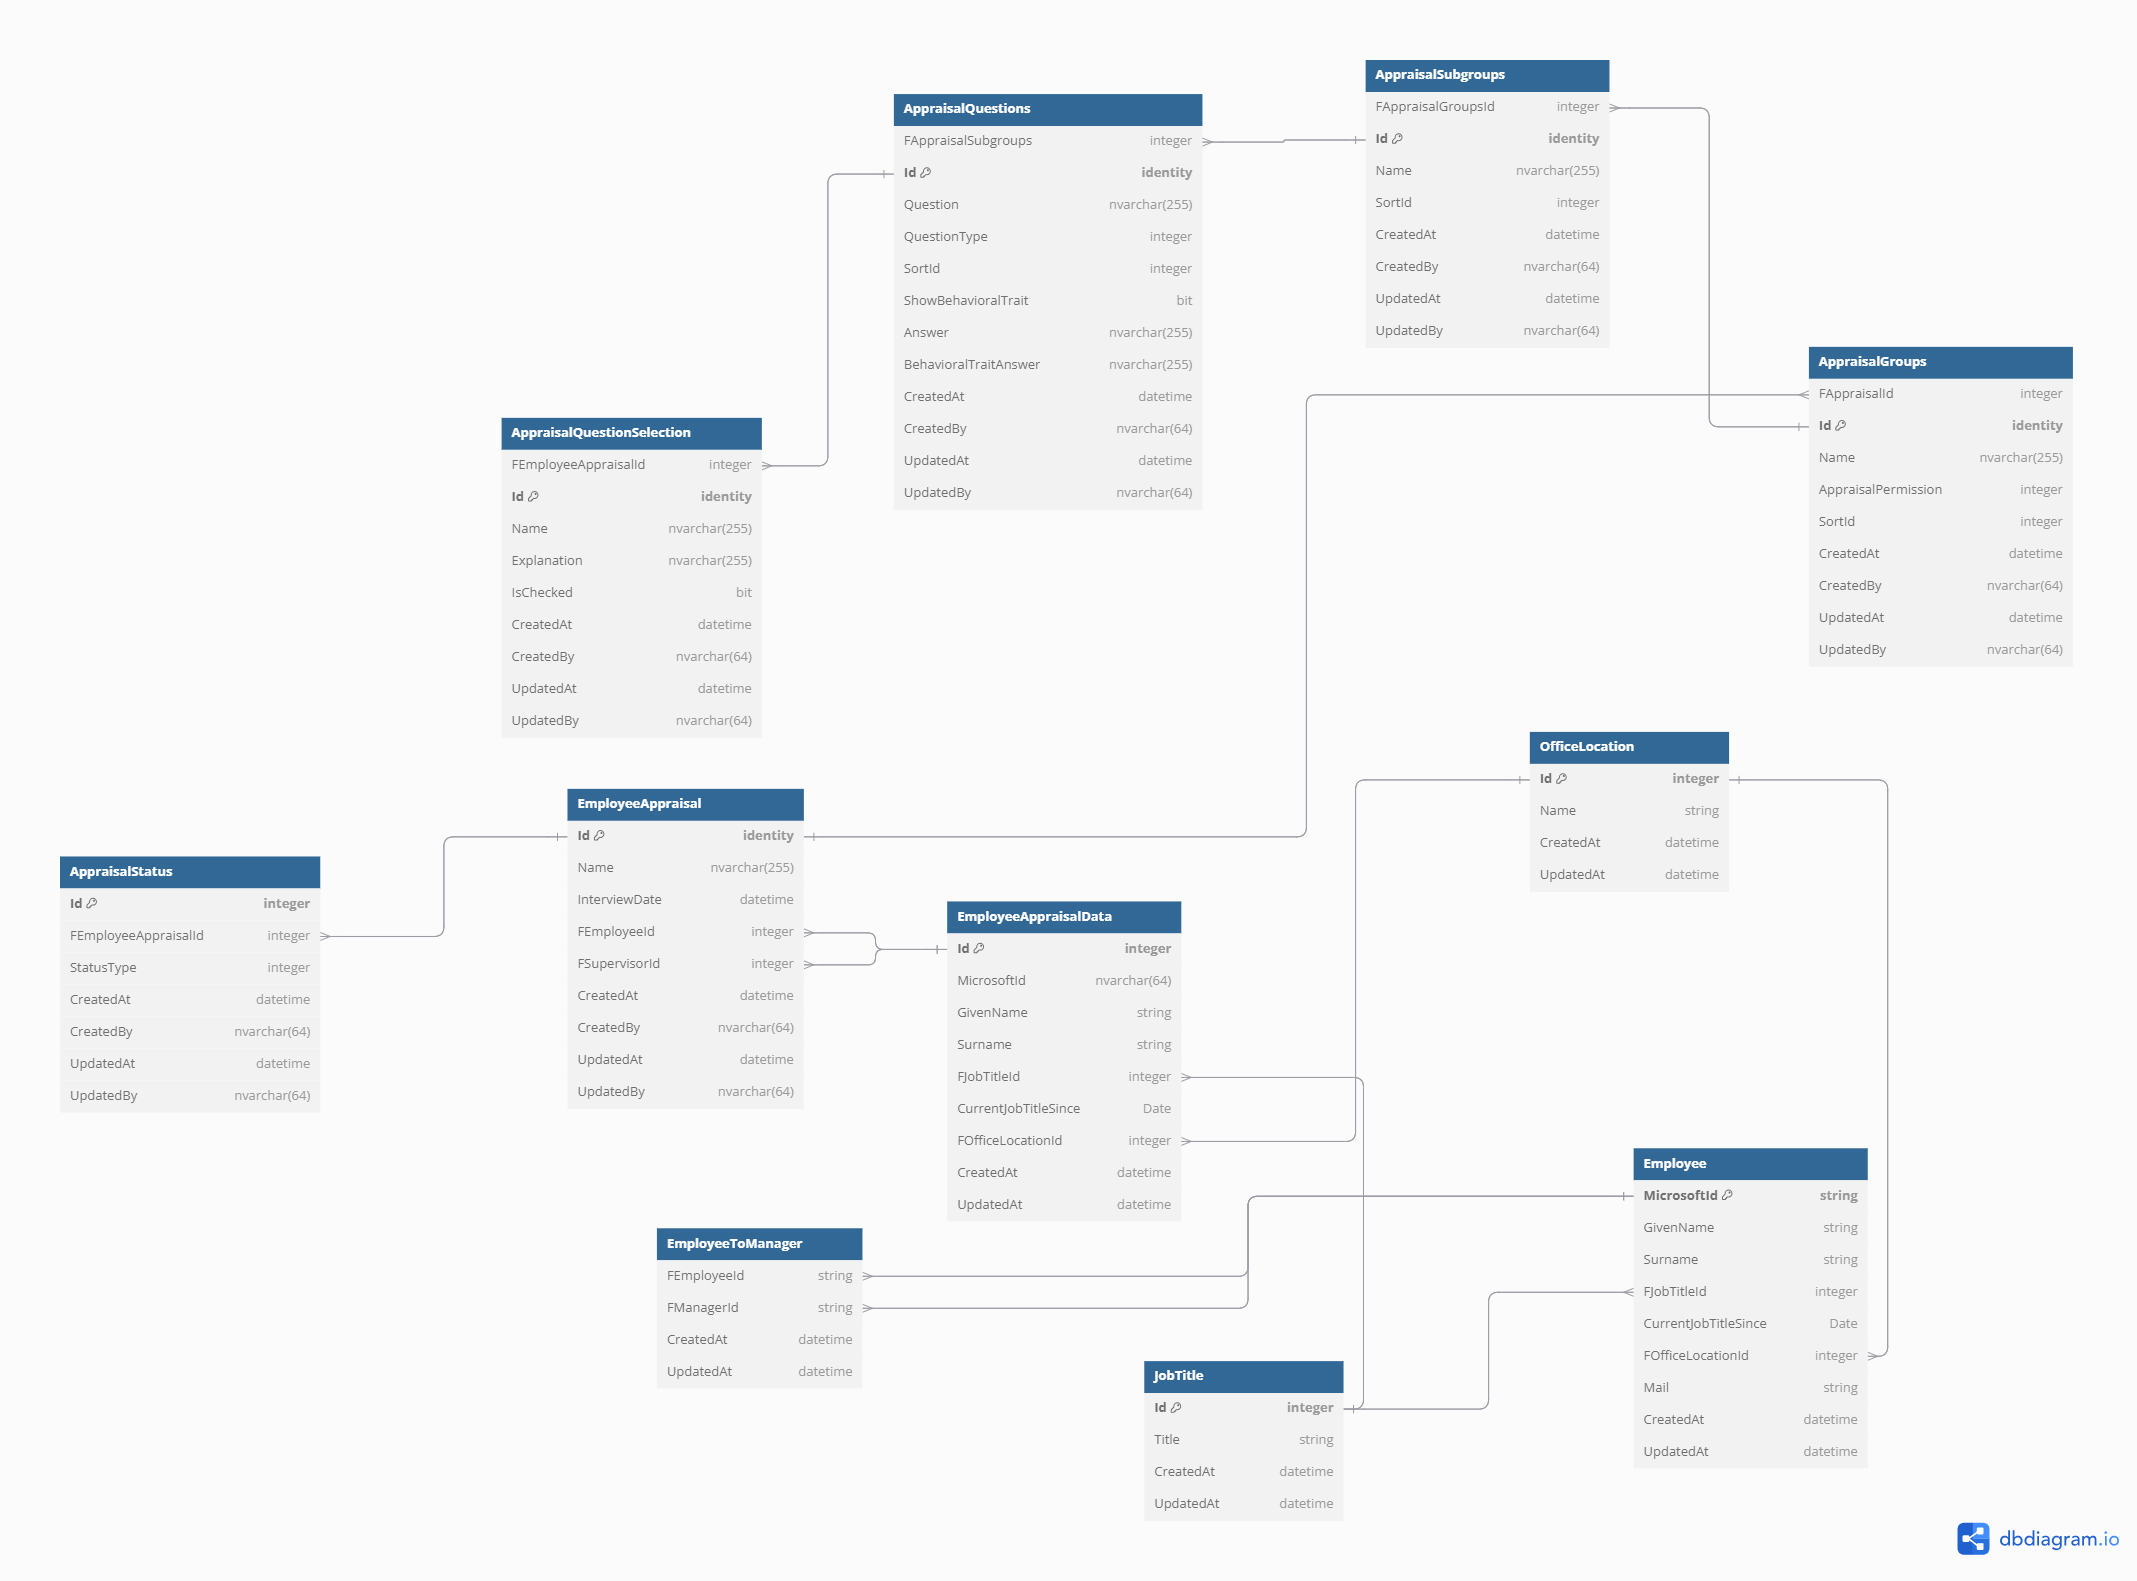
\includegraphics[width=0.8\textwidth]{images/er_modell_design.png}
    \caption{ER-Diagramm der Datenbankstruktur.}
    \label{fig:db_er_model}
\end{figure}

\section{Workflows}
Die Konzeption des Systems umfasst klar definierte Workflows, um eine reibungslose Funktionalität und Effizienz sicherzustellen:
\begin{itemize}
    \item \textbf{Datenimport:} Mitarbeitendengesprächsdaten werden über das Backend in die relationale Datenbank importiert. Hierbei wird eine automatische Validierung der Eingabedaten durchgeführt, um die Datenqualität sicherzustellen.
    \item \textbf{Datenverarbeitung:} Geplante Hintergrundjobs übernehmen Aufgaben wie die Berechnung aggregierter Statistiken, das Generieren von Berichten oder das Versenden von Benachrichtigungen an berechtigte Benutzer.
    \item \textbf{Visualisierung:} Die aufbereiteten Daten werden über definierte RESTful APIs an das Frontend übermittelt, wo sie durch interaktive Diagramme wie Donut- und Radarcharts anschaulich dargestellt werden.
\end{itemize}

\section{Sicherheitskonzepte}
Die Sicherheit des Systems wird durch mehrere bewährte Maßnahmen gewährleistet, um Datenintegrität und Vertraulichkeit sicherzustellen:
\begin{itemize}
    \item \textbf{Authentifizierung:} Benutzer authentifizieren sich über Azure Active Directory (AAD), das Multi-Faktor-Authentifizierung und Single Sign-On (SSO) unterstützt.
    \item \textbf{Datenverschlüsselung:} Alle sensiblen Daten, sowohl im Ruhezustand als auch während der Übertragung, werden durch moderne Verschlüsselungsmethoden wie AES-256 geschützt.
    \item \textbf{Rechteverwaltung:} Eine fein granulierte, rollenspezifische Zugriffskontrolle (RBAC) stellt sicher, dass nur autorisierte Benutzer auf spezifische Daten und Funktionen zugreifen können.
\end{itemize}

\section{Zusammenfassung}
Die vorgestellte Konzeption kombiniert innovative Technologien, effiziente Workflows und umfassende Sicherheitsmaßnahmen, um eine performante und skalierbare Lösung für die Verwaltung und Visualisierung von Mitarbeitendengesprächsdaten zu gewährleisten. Durch den gezielten Einsatz moderner Entwicklungs- und Sicherheitsstandards wird eine benutzerfreundliche und zuverlässige Plattform geschaffen, die den Anforderungen sowohl auf technischer als auch auf organisatorischer Ebene gerecht wird.

